%%%%%%%%%%%%%%%%%%%%%%%%%%%%%%%%%%%
\subsection{Cryogenic Internal Piping}
\label{sec:fdgen-slow-cryo-int-piping}
\label{sec:fdsp-slow-cryo-int-piping}
\label{sec:fddp-slow-cryo-int-piping}
% david m

% some text below adapted from D. Montanari, et al, "Overview of the Long-Baseline Neutrino Facility Cryogenic System", DOI: 10.18462/iir.cryo.2017.033

The cryogenic internal piping comprises several manifolds to
distribute the liquid and gaseous argon inside the cryostat during all
phases ({\em e.g.}, gaseous purge, liquid distribution, cool down) and
various pipe stands to return argon to the outside ({\em e.g.}
boil-off gaseous argon).  Vacuum insulated pipe stands are needed to
transition from inside to outside in a way that does not affect the
purity and does not introduce a significant heat load.

LBNF has the expertise for engineering design and installation of the
detector internal piping, while the CISC consortium has the expertise
on the physics requirements, the relevant risk registries, and the
interfaces with other detector systems. Ultimate responsibility for
costing the internal cryogenic piping system also lies with the CISC
consortium. It is important for these two groups to interact closely
to ensure that the system will allow us to achieve the physics we
need, avoid interference with other detector systems, and mitigate
risks.

We have formed a Cryogenics Systems working group with conveners from
both the CISC consortium and LBNF. This group will have both LBNF and
CISC members and provide an official forum where we interface and
establish the final design.

The initial design for the cryogenic internal piping calls for some
\SI{750}{m} of pipe per cryostat for purging and filling, laid out as
shown in Fig.~\ref{fig:fd-slow-cryo-int-piping}-Left, and 20 flange-pipes assemblies, as the one shown
on the right pannel of Fig.~\ref{fig:fd-slow-cryo-int-piping}, with a CF DN250 flange penetrated by two $\sim$ \SI{2.2}{m} long pipes.

\begin{dunefigure}[Cryogenic internal piping]{fig:fd-slow-cryo-int-piping}
  {Left: Cryogenic internal piping for purging (red) and filling (blue). Right: Cool-down pipes, LAr in blue (vacuum jacketed) and GAr in red. }
  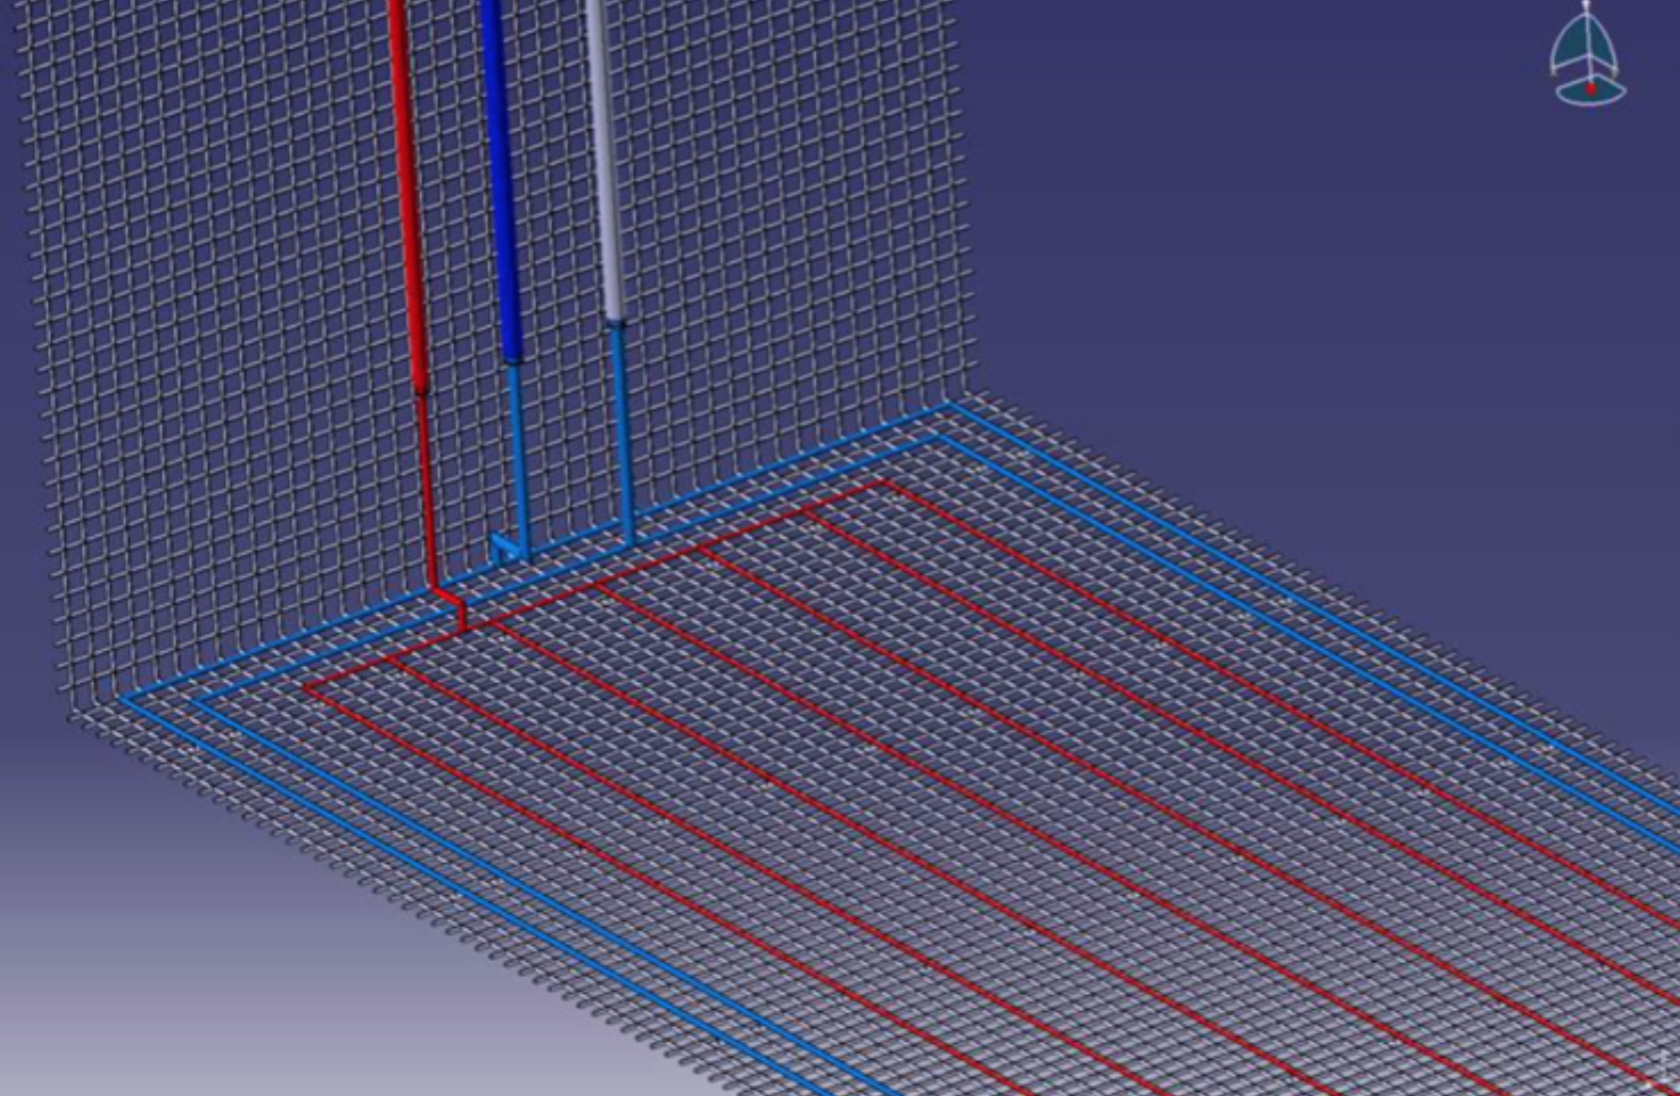
\includegraphics[height=0.3\textwidth]{DUNE-CryoIntPiping}
  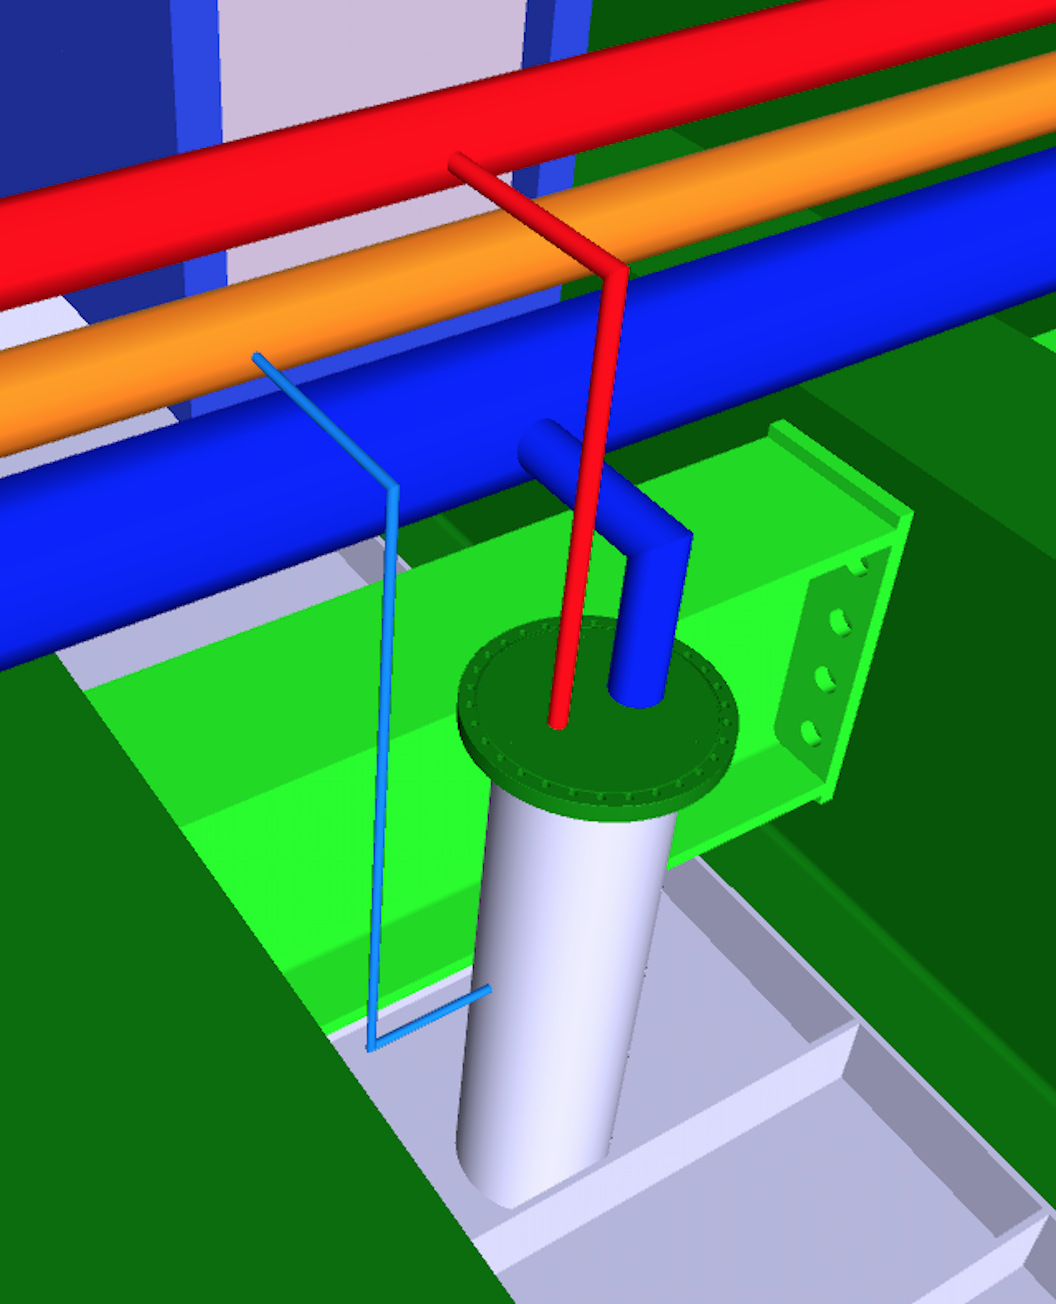
\includegraphics[height=0.3\textwidth]{cisc_CoolDownPipes.png}
\end{dunefigure}



% Below is some detailed design and transpo text to keep for the TDR
%
%We are talking about almost 300 m of 3” pipe and almost 450 m of 2” pipes, they will take some space.
%The majority of them could probably be transported in bunches. Assuming 6 m as long sections, there would be 50 of 3” pipe and 75 of 2” pipe.
%I can see them packing together 10-15 6-m long sections, which will give us 5 pallets/boxes each (assuming 10 sections of the 3” and 15 of the 2”).
%Each one would be about 6.2 m long x 0.8 m wide x 0.5 m high. They could also just bundle the pipes together, but I think they would still sit on a
%pallet even in this case. These would need to be delivered to the site, stored, transported down, and stored again before they are used.
%Depending on when they are installed they could (or not) be stored inside the cryostat itself or in one of the drifts (assuming that CF is fine with that).

%Then there are the 20 cool down pipes for the top. Those are easier: they are CF DN250, so the OD of the flange is 304 mm.
%The length may vary depending on the height of the feedthrough, but shouldn’t be more than ~2.2 m. The box could be something like 2.6 m x 0.6 m x 0.6 m. 20 of them.
%They could probably be a little smaller, but I am not in the shipping industry. This is just a ROM. They could also put many of them in the same box and save space,
%but they will soon run into shaft limits. These would need to be delivered to the site, stored, transported down, and stored again before they are used.
%The last step could take place on top of the cryostat.
